\documentclass[12pt, a4paper, oneside]{article}
\usepackage{amsmath, amsthm, amssymb, bm, graphicx, hyperref, mathrsfs, zhnumber}

% Chinese
\usepackage{CJKutf8}

\title{\vspace{-3.3cm}\textbf{高级宏观经济学作业一}}
\author{邓皓天\quad 2023310114}
\date{}
\linespread{2}
\newcounter{problemname}
\newcounter{answername}
\newenvironment{problem}{\stepcounter{problemname}\par\noindent\textbf{}}{\\\par}
\newenvironment{answer}{\stepcounter{answername}\par\noindent\textbf{答:}\newline}{\\\par}


\begin{document}
\begin{CJK*}{UTF8}{gbsn}
\maketitle

\begin{problem}
	一、在索洛模型中考虑财政政策。假设生产函数$Y(t)=F(K(t), A(t) L(t))$满足索洛模型的基本假设。
	政府消费为$G(t)$,资金来源为总额税$T(t)$,每期预算平衡。
	储蓄为可支配收入的固定比例,储蓄率为$s$。
	\begin{enumerate}
		\item 写出总资本的运动方程。
		\item 写出单位有效工人平均资本的运动方程。(令$g(t) \equiv \frac{G(t)}{A(t) L(t)}$。)
		\item 假设单位有效工人平均政府消费不随时间变化,即$g(t)=\gamma>0$。作图说明模型可能存在多重均衡并判断不同均衡点是否是稳定的。
		\item 请根据稳态条件推导,政府消费增加会让稳态资本存量、产出、消费分别如何变化?(提示:判断$\frac{\partial k^{*}}{\partial \gamma}$的符号)
	\end{enumerate}
	\
\end{problem}
\begin{answer}
\noindent
1. 
$
Y= C+ I+ G = C+ S +T \quad \Rightarrow \quad I=S \quad(T=G)
\\
\dot{K}(t)=I(t)-\delta K(t)=S \cdot[Y(t)-T(t)]-\delta K(t)=S \cdot[Y(t)-G(t)]-\delta K(t)
$

\noindent
2.
$
k=\frac{K}{A L} \quad \Rightarrow \quad \frac{d k}{d t}=\frac{1}{(A L)^{2}}\left[\frac{d K}{d t} \cdot A L-K \cdot\left(A \cdot \frac{d L}{d t}+L \cdot \frac{d A}{d t}\right)\right]
$

$
\begin{aligned} \dot{k}(t) & =\frac{\dot{K}(t)}{A(t) L(t)}-k(t) \cdot\left[\frac{1}{L(t)} \cdot \frac{d L}{d t}+\frac{1}{A(t)} \cdot \frac{d A}{d t}\right] \\ & =\frac{1}{A(t) L(t)}\{S[Y(t)-G(t)]-\delta K(t)\}-(n+g) k(t) \\ & =S \cdot[y(t)-g(t)]-\left(n+g_{A}+\delta\right) k(t)\end{aligned}
$

\noindent
3.当$r=g(t)>0$时,$\dot{k}(t)=s \cdot f[k(t)]-s \gamma-(n+g+\delta) k(t)$。
令$\dot{k}(t)=0$,则$y=f[k(t)]=\gamma+\frac{(n+g+\delta)}{s} k(t)$。
\begin{itemize}
	\item 当$0<k<k_1$时,$r+\frac{(n+g+\delta)}{s} k(t)>f[k(t)]$,$\dot{k}(t)<0$,$k$将降低。
	\item 当$k_1<k<k_2$时,$r+\frac{(n+g+\delta)}{s} k(t)<f[k(t)]$,$\dot{k}(t)>0$,$k$将增加。
	\item 当$k>k_2$时,$r+\frac{(n+g+\delta)}{s} k(t)>f[k(t)]$,$\dot{k}(t)<0$,$k$将降低。
\end{itemize}
\begin{figure}[htpb]
  \begin{center}
    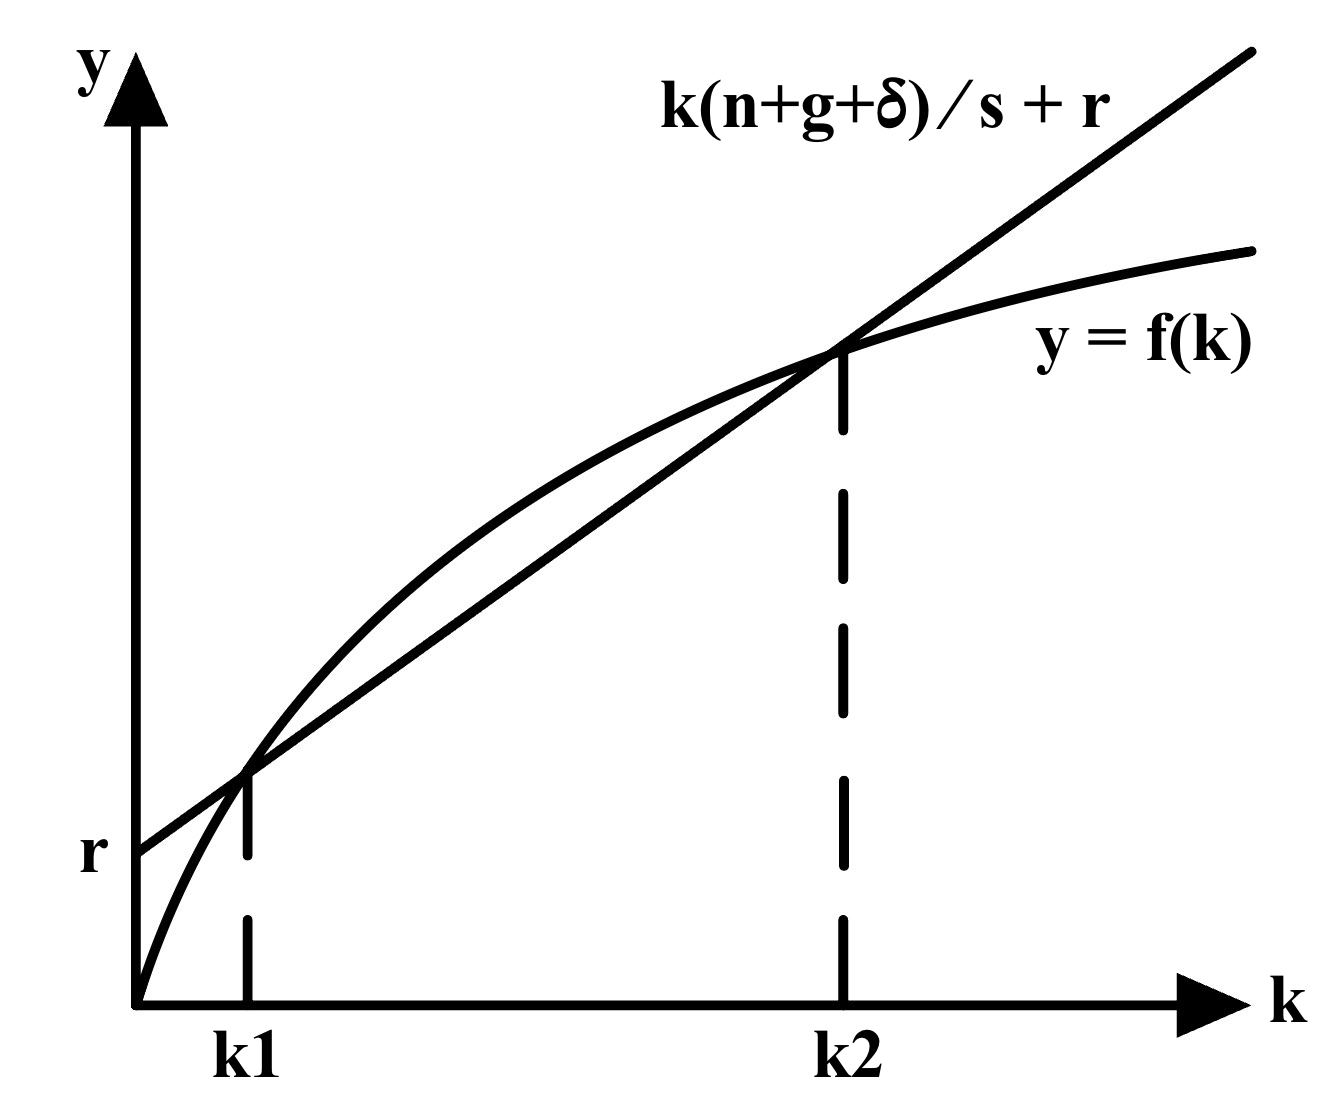
\includegraphics[width=0.6 \linewidth]
    {pic/1_3.png}
  \end{center}
\end{figure}
综上所述,模型可能存在多重均衡,但$k_1$不稳定,$k_2$稳定。

\noindent
4.根据第3题结论可知$f\left[k^{*}(t)\right]=r+\frac{n+g+\delta}{s} \cdot k^{*}(t)$,令$k^{*}=k_2$,等式两侧对$r$求偏导得
$$
f^{\prime}\left[k^{*}(\tau)\right] \cdot \frac{\partial k^{*}}{\partial r}=1+\frac{n+g+\delta}{s} \cdot \frac{\partial k^{*}}{\partial \gamma}
$$
因此可得
$$
\frac{\partial k^{*}}{\partial \gamma}=\frac{1}{f^{\prime}\left[k^{*}(t)\right]-\frac{n+g+\delta}{s}}=\frac{1}{f^{\prime}\left[k^{*}(t)\right]-\beta} \quad, \quad \beta=\frac{n+g+\delta}{s}
$$
在$k=k_2$处,$f^{\prime}\left[k^{*}(t)\right]<\beta$,
因此$\frac{\partial k^{*}}{\partial \gamma}<0$,
又因为$\frac{\partial y}{\partial \gamma}=\frac{\partial y}{\partial k^{*}} \cdot \frac{\partial k^{*}}{\partial \gamma}$,
根据稻田条件有$\frac{\partial y}{\partial k}>0$,
故$\frac{\partial y}{\partial \gamma}<0$。
而$C=(1-S)(y-r)$,所以$\frac{\partial C}{\partial \gamma}=(1-s)\left(\frac{\partial y}{\partial r}-1\right)<0$。

综上,政府消费$\gamma$增加,会让$k^*$、$C$和$y$都减少。
\end{answer}

\begin{problem}
	二、在RCK模型中,假设折旧率$\delta=0$,折现率为$\beta>0$,跨期替代弹性为$\sigma$,人口增长率为 $n$,技术进步率为$g$。假设在BGP上,$g$突然永久性下降。
	\begin{enumerate}
		\item $\dot{c} = 0$曲线和$\dot{k} = 0$曲线会如何变化?
		\item 当$g$下降时,$c$会上升、下降、保持不变还是无法确定?
		\item 假设C—D生产函数$f(k) = k\alpha$,说明$g$的边际变化对BGP上储蓄率的影响(提示:判断 $\frac{\partial s}{\partial g}$的符号)。
	\end{enumerate}
	\
\end{problem}
\begin{answer}
\noindent
1.令$\frac{\dot{C}(t)}{c(t)}=r(t)-n-g-\beta \delta=0$,
$r(t)=f^\prime[k(t)]$。因此$r(t) = n+g+\beta = f^\prime[k(t)]$。
当$g$下降时,$f^\prime[k(t)]$也应下降。由稻田条件可知,$k$会增加,$\dot{c}=0$会右移。
又因为$\dot{k}(t)=w(t)+[r(t)-n-g] k(t)-c(t)=0$,$w(t)=f[k(t)]-k(t) \cdot f[k(t)]$,
因此$C(t)=f[k(t)]-k(t) \cdot f^{\prime}[k(t)]+k(t) \cdot f^{\prime}[k(t)]-(n+g) k(t)=f[k(t)]-(n+g) k(t)$,当$g$下降时,$C(t)$会增加。

\noindent
2.$k_t$的变动由$k_{t-1}$决定,存在一定粘性,
而$C$的变动为刚性变动,但由于无法确定新旧均衡点的推对位置,故无法确定。

\noindent
3.根据C-D生产函数可知$y=f(k)=k^{\alpha}$,因此$f^{\prime}(k)=n+g+\beta=\alpha k^{\alpha-1}$
$$1=\alpha(\alpha-1) k^{\alpha-2} \cdot \frac{\partial k}{\partial g} \Rightarrow \frac{\partial k}{\partial g}=\frac{1}{\alpha(\alpha-1) k^{\alpha-2}}
$$
$$
\begin{aligned} c & =k^{\alpha}-(n+g) k \\ S & =\frac{y-c}{y}=\frac{(n+g) k}{k^{\alpha}}=\frac{n+g}{k^{\alpha-1}} \\ \frac{\partial S}{\partial g} & =\frac{1 \cdot k^{\alpha-1}-(n+g)(\alpha-1) k^{\alpha-2} \cdot \frac{\partial k}{\partial g}}{\left(k^{\alpha-1}\right)^{2}}=\frac{k^{\alpha-1}-(n+g) \cdot \frac{1}{\alpha}}{k^{2 \alpha-2}}\\&=\frac{\alpha k^{\alpha-1}-(n+g)}{\alpha k^{2 \alpha-2}}=\frac{\beta}{\alpha\left(k^{2-1}\right)^{2}}>0\end{aligned}
$$
综上所述,$g$的变化会使BGP上的储蓄率$s$同向变化。
\end{answer}

\begin{problem}
	三、资源的有限性。假设生产函数为$Y=K^{\alpha}(A L)^{\beta} R^{1-\alpha-\beta}$,
	其中$\alpha>0$,$\beta>0$且$\alpha+\beta<1$。资本存量的变动方程为:$\dot{K}=s Y-\delta K$。假设技术进步率和人口增长率分别为$g$和$n$。$R$代表总量有限的自然资源,增长率为$0$。
	\begin{enumerate}
		\item 该经济是否有唯一的平衡增长路径?如果有,$Y$和$K$的增长率分别是多少?
		该路径是否稳定?如果没有,请解释原因。
		\item 自然资源总量有限是否意味着人均收入的增长最终必然会停滞?
	\end{enumerate}
	\
\end{problem}
\begin{answer}
\noindent
1.如果存在BGP,则$\frac{\dot{K}}{K}$为常数。又由于$\frac{\dot{K}}{K}=s \cdot \frac{Y}{K}-\delta$,意味着$\frac{Y}{K}$为常数,即$\frac{d \ln Y}{d t}=\frac{d \ln K}{d t}=g$。
又由于$Y=K^{\alpha}(A L)^{\beta} \cdot R^{1-\alpha-\beta}$,因此
$$
\begin{aligned} \ln Y & =\alpha \ln K+\beta(\ln A+\ln L)+(1-\alpha-\beta) \ln R \\ \frac{d \ln Y}{d t} & =\alpha \cdot \frac{d \ln K}{d t}+\beta\left(g_{A}+n\right) \Rightarrow g_{Y}=\alpha g_{K}+\beta\left(g_{A}+n\right) \\ g^{*} & =\frac{\beta\left(n+g_{A}\right)}{1-\alpha}\end{aligned}
$$
\begin{itemize}
	\item 如果$g_Y>g_K$,则$\frac{Y}{K}$增加,$\frac{\dot{K}}{K}$上升,直到$g_Y=g_K$。
	\item 如果$g_Y<g_K$,则$\frac{Y}{K}$减少,$\frac{\dot{K}}{K}$下降,直到$g_Y=g_K$。
\end{itemize}
综上所述,存在BGP。

\noindent
2.
$$
\begin{array}{l}Y=K^{\alpha}(A L)^{\beta} R^{1-\alpha-\beta} \\ g_{\frac{Y}{L}}=g_{Y}-g_{L}=g^{*}-n=\frac{\beta\left(n+g_{A}\right)}{1-\alpha}-n=\frac{\beta\left(n+g_{A}\right)-n+n \alpha}{1-\alpha}=\frac{n(\beta-1+\alpha)+\beta g_{A}}{1-\alpha}=\frac{\beta g_{A}-(1-\beta-\alpha) n}{1-\alpha}\end{array}
$$
令$g_{\frac{Y}{L}}=0$,则$g_{A}=\frac{(1-\alpha-\beta) n}{\beta}=\Delta$,
当$g_A>\Delta$时,人均产出将增长,反之则下降。
\end{answer}
\begin{problem}
	四、在标准的RCK模型中,假设生产函数为$f(k)=k^{\alpha}$,资本折旧率为$\delta$,
	从而资本积累方程变为$\dot{k}(t)=f(k(t))-(n+g+\delta) k(t)-c(t)$。
	\begin{enumerate}
		\item 请写出社会计划者的最优化问题和期值哈密尔顿函数。
		\item 求解最优化问题的一阶条件。
		\item 在稳态附近对$\dot{c}(t)$和$\dot{k}(t)$取一阶泰勒近似,推导线性微分方程系统的系数矩阵$\Delta$并计算其特征值。
		\item 假设中美两国经济的模型参数如下表所示,请使用计算器计算中美两国经济向稳态收敛的速度。
		$$
		\begin{array}{ccccccc}\\\hline & \theta & n & g & \beta & \delta & \alpha \\\hline \text{中国} & 1 & 1 \% & 1 \% & 0.04 & 10 \% & 0.5 \\\text{美国} & 1 & 1 \% & 1 \% & 0.01 & 4 \% & 1 / 3 \\\hline\\\end{array}
		$$
	\end{enumerate}
	\
\end{problem}
\begin{answer}
\noindent
1.
$$
\begin{array}{ll}\max & U(0)=\int_{0}^{\infty} e^{-\beta t} \frac{C(t)^{1-\theta}}{1-\theta} d t \\ \text { s.t. } & \dot{k}(t)=k^{\alpha}(t)-(n+g+\delta) k(t)-C(t) \\ & k(0)>0, \quad \lim _{t \rightarrow \infty} e^{-R(t)+(n+g+\delta) t} k(s) \geqslant 0 \\ H= & \frac{c(t)^{1-\theta}}{1-\theta}+\lambda(t)\left[k^{\alpha}(t)-(n+g+\delta) k(t)-C(t)\right]\end{array}
$$

\noindent
2.
$$
\begin{array}{l}\frac{\partial H}{\partial C}=0 \Rightarrow C(t)^{-\theta}=\lambda(t) \quad \Rightarrow \quad \frac{\dot{\lambda}(t)}{\lambda(t)}=-\theta \cdot \frac{\dot{C}(t)}{C(t)} \\ \frac{\partial H}{\partial k}+\dot{\lambda}(t)=\beta \lambda \Rightarrow \lambda(t)\left[\alpha k^{\alpha-1}(t)-(n+g+\delta)\right]-\theta \cdot \frac{\dot{C}(t)}{C(t)} \cdot \lambda(t)=\beta \cdot \lambda(t) \\ \frac{\dot{C}(t)}{C(t)}=\frac{\alpha k^{\alpha-1}(t)-(n+g+\delta+\beta)}{\theta} \\ \lim _{t \rightarrow \infty} e^{-\beta t} \lambda(t) \cdot k(t)=0\end{array}
$$
\noindent
3.
$$
\begin{array}{l}\left.\begin{array}{l}\dot{c}(t)=\left[\alpha k^{\alpha-1}(t)-(n+g+\delta+\beta)\right] \cdot \frac{C(t)}{\theta} \\ \dot{k}(t)=k^{\alpha}(t)-(n+g+\delta) k(t)-C(t)\end{array}\right\} \Rightarrow \begin{array}{l}\alpha k^{\alpha-1}(t)=n+g+\delta+\beta \\ c(t)=k^{\alpha}(t)-(n+g+\delta) k(t)\end{array} \\ {\left[\begin{array}{l}\dot{k}(t) \\ \dot{c}(t)\end{array}\right] \simeq\left[\begin{array}{ll}\frac{\partial \dot{k}}{\partial k} & \frac{\partial \dot{k}}{\partial C} \\ \frac{\partial \dot{c}}{\partial k} & \frac{\partial \dot{C}}{\partial C}\end{array}\right]\left[\begin{array}{l}k-k^{*} \\ c-c^{*}\end{array}\right]=\Delta\left[\begin{array}{l}k-k^{*} \\ c-c^{*}\end{array}\right]} \\\end{array}
$$
$$
\begin{array}{l}\frac{\partial \dot{k}}{\partial k}=\alpha k^{\alpha-1}(t)-(n+g+\delta)=\beta \\ \frac{\partial \dot{k}}{\partial c}=-1 \\ \frac{\partial \dot{C}}{\partial k}=\frac{C(t)}{\theta} \cdot \alpha(\alpha-1) k^{\alpha-2}(t) \\ \frac{\partial \dot{C}}{\partial c}=\frac{1}{\theta}\left[\alpha k^{\alpha-1}-(n+g+\delta+\beta)\right]=0\end{array}
$$
$$
\Delta=\left[\begin{array}{cc}\beta & -1 \\ \frac{C(t)}{\theta} \alpha \cdot(\alpha-1) k^{\alpha-2}(t) & 0\end{array}\right] \quad \begin{array}{l}\operatorname{tr}(\Delta)=\beta>0 . \\ |\Delta|=\frac{C(t)}{\theta} \alpha \cdot(\alpha-1) k^{\alpha-2}(t)<0\end{array}
$$
设$\lambda_1>0$,$\lambda_2<0$。
解方程
$$
\lambda^{2}-\beta \lambda+\frac{C(t)}{\theta} \alpha(\alpha-1) k^{\alpha-2}(t)=0
$$
解得
$$\lambda_{1}=\frac{\beta+\sqrt{\beta^{2}-\frac{4 C(t)}{\theta} \alpha(t-1) k^{\alpha 2}(t)}}{2} \quad \lambda_{2}=\frac{\beta-\sqrt{\left.\beta^{2}-\frac{4 C(t)}{\theta} \alpha(t)\right) k^{\alpha-2}(t)}}{2}$$
\noindent
4.
中国
$$
\begin{array}{l}\left.\begin{array}{ll}\frac{1}{2 \sqrt{k}} & =0.16 \\ C(t) & =\sqrt{k}-0.12 k\end{array}\right\} \Rightarrow \begin{array}{l}k^{*}=9.765652 \\ C^{*}=1.953125\end{array} \\ \lambda=\frac{0.04 \pm \sqrt{0.04^{2}-\frac{4 c}{1} \cdot 0.5(-05) \cdot k^{-1.5}}}{2} \Rightarrow \quad \lambda_{1} \approx 0.1481 \quad \lambda_{2} \approx-0.1081 \\\end{array}
$$
美国
$$
\begin{array}{l}\left.\begin{array}{l}\frac{1}{2 \sqrt{k}}=0.07 \\ C(t)=\sqrt{k}-0.06 k\end{array}\right\} \Rightarrow \begin{array}{l}k^{*}=51.020408 \\ C^{*}=4.081633\end{array} \\ \lambda=\frac{0.01 \pm \sqrt{0.01^{2}-\frac{4 C}{1} \cdot(-0.25) k^{-15}}}{2} \Rightarrow \lambda \approx 0.01065 \quad \lambda_{2} \approx 0.00065 \\\end{array}
$$
\end{answer}
\end{CJK*}
\end{document}